\begin{frame}[fragile,t]
\frametitle{\hfill}
\MyHeading{Why \ED?}
\vspace{\mytopbit}
{Example: Fine structure of aurora in real time}
% \begin{center}
%   \movie[width=0.5\columnwidth,showcontrols]{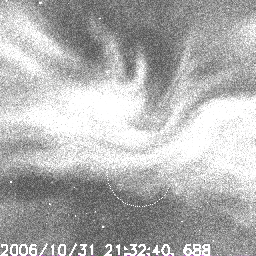
\includegraphics[width=0.5\columnwidth]{ask-eiscat}}{swirls.avi}
% \end{center}

\begin{center}
% \href{run:/usr/bin/mplayer -fs swirls.avi}{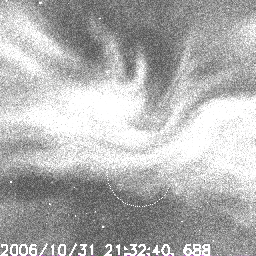
\includegraphics[width=0.5\columnwidth]{ask-eiscat}}
% For laptop version
% \href{run:/usr/bin/gnome-mplayer --ss 0 --fullscreen  swirls.avi}{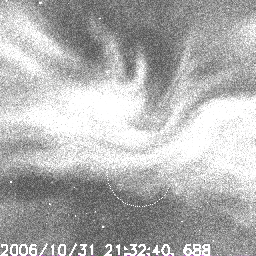
\includegraphics[width=0.5\columnwidth]{ask-eiscat}}
% For ISGC website
% 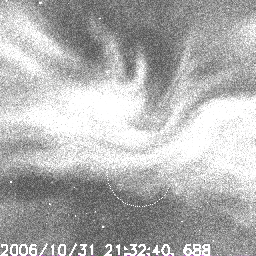
\includegraphics[width=0.5\columnwidth]{ask-eiscat}
% original move command possibly could be used with M$ products?
% \movie[width=0.5\columnwidth,showcontrols]{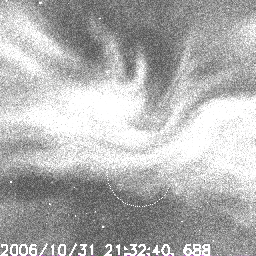
\includegraphics[width=0.5\columnwidth]{ask-eiscat}}{swirls.avi}
\movie[width=0.5\columnwidth,showcontrols]{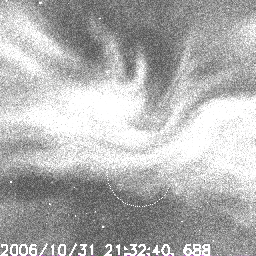
\includegraphics[width=0.5\columnwidth]{ask-eiscat}}{swirls.wmv}
\end{center}

{\colblack \scriptsize \it ASK 3$\times$3 degrees 31 Oct 2006 Hanna Dahlgren, KTH} \\
\end{frame}
